\subsection{EU Nuclear Operation until 2050}

\begin{frame}
	\frametitle{Historical Operation of EU Reactors}
	
\begin{table}[h]
	\centering
%	\scalebox{0.86}{
		\begin{tabular}{cccc}
			\hline
			\textbf{Category } & \textbf{Value} & \textbf{Unit} & \textbf{Specifics}\\ \hline
			Total UOX Usage  & 181,471 & MTHM &  \\ 
			Total MOX Usage  & 6,302 & MTHM & \\ 
			Total Used UOX Stored  & 141,659 & MTHM & \gls{UNF} that is not reprocessed\\ 
			Total Used  MOX Stored  & 3,611 & MTHM & \gls{UNF} that is not reprocessed \\ 
			Total Tailings  & 1,081,826 & MTHM & \\ 
			Total Natural U Used  & 1,269,897 & MTHM & \\ \hline
		\end{tabular}
		\caption{Simulation Results for Historical Nuclear Operation of \gls{EU} Nations}
		\label{tab:sim_result}
\end {table}

\end{frame}

\begin{frame}
	\frametitle{Tails and UNF Inventory}
\begin{figure}[htbp!]
\begin{minipage}[b]{.45\linewidth}
	\begin{center}
		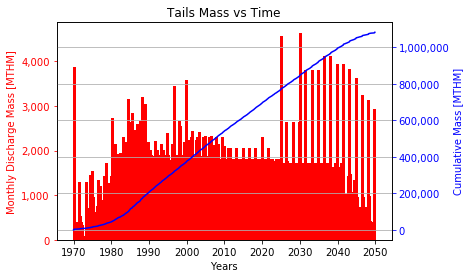
\includegraphics[width=\textwidth]{./images/eu_future/tails.png}
	\end{center}
	\caption{Timeseries of Tails Mass in the \gls{EU}.}
	\label{fig:eu_tail}
\end{minipage}
\hspace{.5cm}
\begin{minipage}[b]{.45\linewidth}
	\centering
	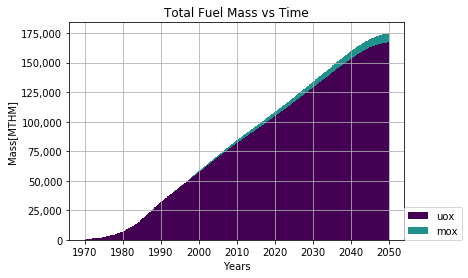
\includegraphics[width=\textwidth]{./images/eu_future/total_fuel.png}
	\caption{Timeseries of Total Fuel Usage in \gls{EU}.}
	\label{fig:eu_fuel}
\end{minipage}
\end{figure}
\end{frame}

\begin{frame}

\begin{figure}[htbp!]
	\begin{center}
			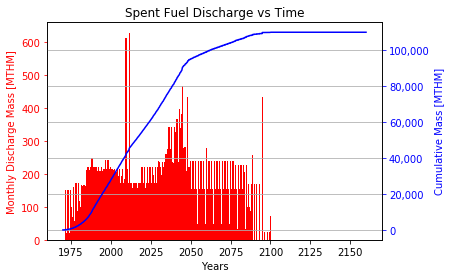
\includegraphics[scale=0.7]{./images/eu_future/snf_discharge.png}
	\end{center}
	\caption{Timeseries of Used Nuclear Fuel in \gls{EU}.}
	\label{fig:eu_snf}
\end{figure}

\end{frame}

\begin{frame}
	\frametitle{Plutonium in Legacy UNF}
	
\begin{table}[h]
	\centering
	\begin{tabular}{ccc}
		\hline
		\textbf{Isotope} & \textbf{Mass Fraction in Used Fuel [\%]} & \textbf{Quantity [t]} \\ \hline
		Total & 0.9358 & 1,325 \\ 
		Pu238 & 0.0111 & 15.72 \\ 
		Pu239 & 0.518 & 733.79 \\ 
		Pu240 & 0.232 & 328.64 \\ 
		Pu241 & 0.126 & 178.49 \\ 
		Pu242 & 0.0487 & 68.98 \\ \hline
	\end{tabular}
	\caption{Plutonium From Used Fuel}
	\label{tab:pu}
\end{table}
\end{frame}


\subsection{French Transition Scenario ~2160}

\begin{frame}
	\frametitle{SFR Deployment with Legacy UNF}
	\begin{itemize}
		\item Reprocessing UNF from all EU nations can start approx. 270 SFRs.
		\item Two generations of 66GWe SFRs = 220 SFRs
		\item Breeding Ratio of SFRs over one. ($\frac{12.6}{11.0} = 1.145$)
		\item Initial Pu loading of $4.9$ tons for ASTRID-type SFR \cite{marsaultmarie-sophie_pre-conceptual_2012}.
		\item $\frac{Pu \ from \ legacy \ \gls{UNF}}{4.9} \approx 270$
	\end{itemize}
\end{frame}

\begin{frame}
	\frametitle{Frech Transition Results}
	
\begin{table}[h]
	\centering
	\scalebox{0.86}{
		\begin{tabular}{ccc}
			\hline
			\textbf{Category} & \textbf{Unit} & \textbf{Value}  \\ \hline
			Total MOX used & MTHM & 127,640  \\ 
			Total \glspl{SFR} Deployed & & 220 \\ 
			Total Plutonium Reprocessed & MTHM & 16,352 \\ 
			Total MOX from UOX Waste & MTHM & 6,570  \\ 
			Total MOX from MOX Waste & MTHM  & 121,070 \\ 
			Total Tails used & MTHM & 116,153 \\ 
			Total legacy UNF reprocessed & MTHM & 77,082 \\ 
			Total Reprocessed Uranium Stockpile & MTHM & 184,172 \\ 
			Total Reprocess Waste & MTHM & 16,352 \\ \hline
		\end{tabular}}
		\caption {\gls{SFR} Simulation Results}
		\label{tab:sfr_sim_result}
\end {table}


\end{frame}

\begin{frame}
	\frametitle{Material Flow in French Transition Scenario}
	
\begin{figure}[htbp!]
\begin{minipage}[b]{.45\linewidth}
	\begin{center}
		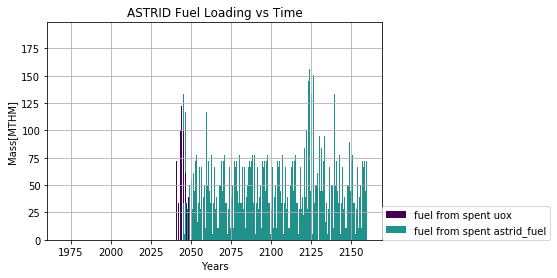
\includegraphics[width=\textwidth]{./images/french-transition/where_fuel.png}
	\end{center}
	\caption{Timeseries of fuel loaded into \glspl{SFR}}
	\label{fig:fuel}
\end{minipage}
\hspace{.5cm}
\begin{minipage}[b]{.45\linewidth}
	\centering
		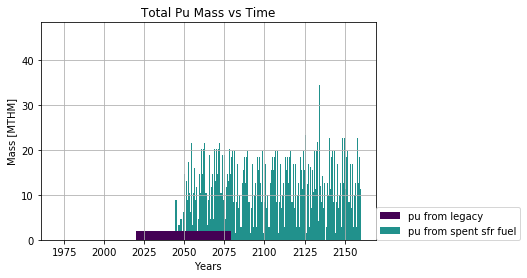
\includegraphics[width=\linewidth]{./images/french-transition/pu.png}
	\caption{Separated plutonium discharge from Reprocessing Plant}
	\label{fig:pu_no_cum}
\end{minipage}
\end{figure}

\end{frame}
	
	